\documentclass[1p]{elsarticle_modified}
%\bibliographystyle{elsarticle-num}

%\usepackage[colorlinks]{hyperref}
%\usepackage{abbrmath_seonhwa} %\Abb, \Ascr, \Acal ,\Abf, \Afrak
\usepackage{amsfonts}
\usepackage{amssymb}
\usepackage{amsmath}
\usepackage{amsthm}
\usepackage{scalefnt}
\usepackage{amsbsy}
\usepackage{kotex}
\usepackage{caption}
\usepackage{subfig}
\usepackage{color}
\usepackage{graphicx}
\usepackage{xcolor} %% white, black, red, green, blue, cyan, magenta, yellow
\usepackage{float}
\usepackage{setspace}
\usepackage{hyperref}

\usepackage{tikz}
\usetikzlibrary{arrows}

\usepackage{multirow}
\usepackage{array} % fixed length table
\usepackage{hhline}

%%%%%%%%%%%%%%%%%%%%%
\makeatletter
\renewcommand*\env@matrix[1][\arraystretch]{%
	\edef\arraystretch{#1}%
	\hskip -\arraycolsep
	\let\@ifnextchar\new@ifnextchar
	\array{*\c@MaxMatrixCols c}}
\makeatother %https://tex.stackexchange.com/questions/14071/how-can-i-increase-the-line-spacing-in-a-matrix
%%%%%%%%%%%%%%%

\usepackage[normalem]{ulem}

\newcommand{\msout}[1]{\ifmmode\text{\sout{\ensuremath{#1}}}\else\sout{#1}\fi}
%SOURCE: \msout is \stkout macro in https://tex.stackexchange.com/questions/20609/strikeout-in-math-mode

\newcommand{\cancel}[1]{
	\ifmmode
	{\color{red}\msout{#1}}
	\else
	{\color{red}\sout{#1}}
	\fi
}

\newcommand{\add}[1]{
	{\color{blue}\uwave{#1}}
}

\newcommand{\replace}[2]{
	\ifmmode
	{\color{red}\msout{#1}}{\color{blue}\uwave{#2}}
	\else
	{\color{red}\sout{#1}}{\color{blue}\uwave{#2}}
	\fi
}

\newcommand{\Sol}{\mathcal{S}} %segment
\newcommand{\D}{D} %diagram
\newcommand{\A}{\mathcal{A}} %arc


%%%%%%%%%%%%%%%%%%%%%%%%%%%%%5 test

\def\sl{\operatorname{\textup{SL}}(2,\Cbb)}
\def\psl{\operatorname{\textup{PSL}}(2,\Cbb)}
\def\quan{\mkern 1mu \triangleright \mkern 1mu}

\theoremstyle{definition}
\newtheorem{thm}{Theorem}[section]
\newtheorem{prop}[thm]{Proposition}
\newtheorem{lem}[thm]{Lemma}
\newtheorem{ques}[thm]{Question}
\newtheorem{cor}[thm]{Corollary}
\newtheorem{defn}[thm]{Definition}
\newtheorem{exam}[thm]{Example}
\newtheorem{rmk}[thm]{Remark}
\newtheorem{alg}[thm]{Algorithm}

\newcommand{\I}{\sqrt{-1}}
\begin{document}

%\begin{frontmatter}
%
%\title{Boundary parabolic representations of knots up to 8 crossings}
%
%%% Group authors per affiliation:
%\author{Yunhi Cho} 
%\address{Department of Mathematics, University of Seoul, Seoul, Korea}
%\ead{yhcho@uos.ac.kr}
%
%
%\author{Seonhwa Kim} %\fnref{s_kim}}
%\address{Center for Geometry and Physics, Institute for Basic Science, Pohang, 37673, Korea}
%\ead{ryeona17@ibs.re.kr}
%
%\author{Hyuk Kim}
%\address{Department of Mathematical Sciences, Seoul National University, Seoul 08826, Korea}
%\ead{hyukkim@snu.ac.kr}
%
%\author{Seokbeom Yoon}
%\address{Department of Mathematical Sciences, Seoul National University, Seoul, 08826,  Korea}
%\ead{sbyoon15@snu.ac.kr}
%
%\begin{abstract}
%We find all boundary parabolic representation of knots up to 8 crossings.
%
%\end{abstract}
%\begin{keyword}
%    \MSC[2010] 57M25 
%\end{keyword}
%
%\end{frontmatter}

%\linenumbers
%\tableofcontents
%
\newcommand\colored[1]{\textcolor{white}{\rule[-0.35ex]{0.8em}{1.4ex}}\kern-0.8em\color{red} #1}%
%\newcommand\colored[1]{\textcolor{white}{ #1}\kern-2.17ex	\textcolor{white}{ #1}\kern-1.81ex	\textcolor{white}{ #1}\kern-2.15ex\color{red}#1	}

{\Large $\underline{12n_{0647}~(K12n_{0647})}$}

\setlength{\tabcolsep}{10pt}
\renewcommand{\arraystretch}{1.6}
\vspace{1cm}\begin{tabular}{m{100pt}>{\centering\arraybackslash}m{274pt}}
\multirow{5}{120pt}{
	\centering
	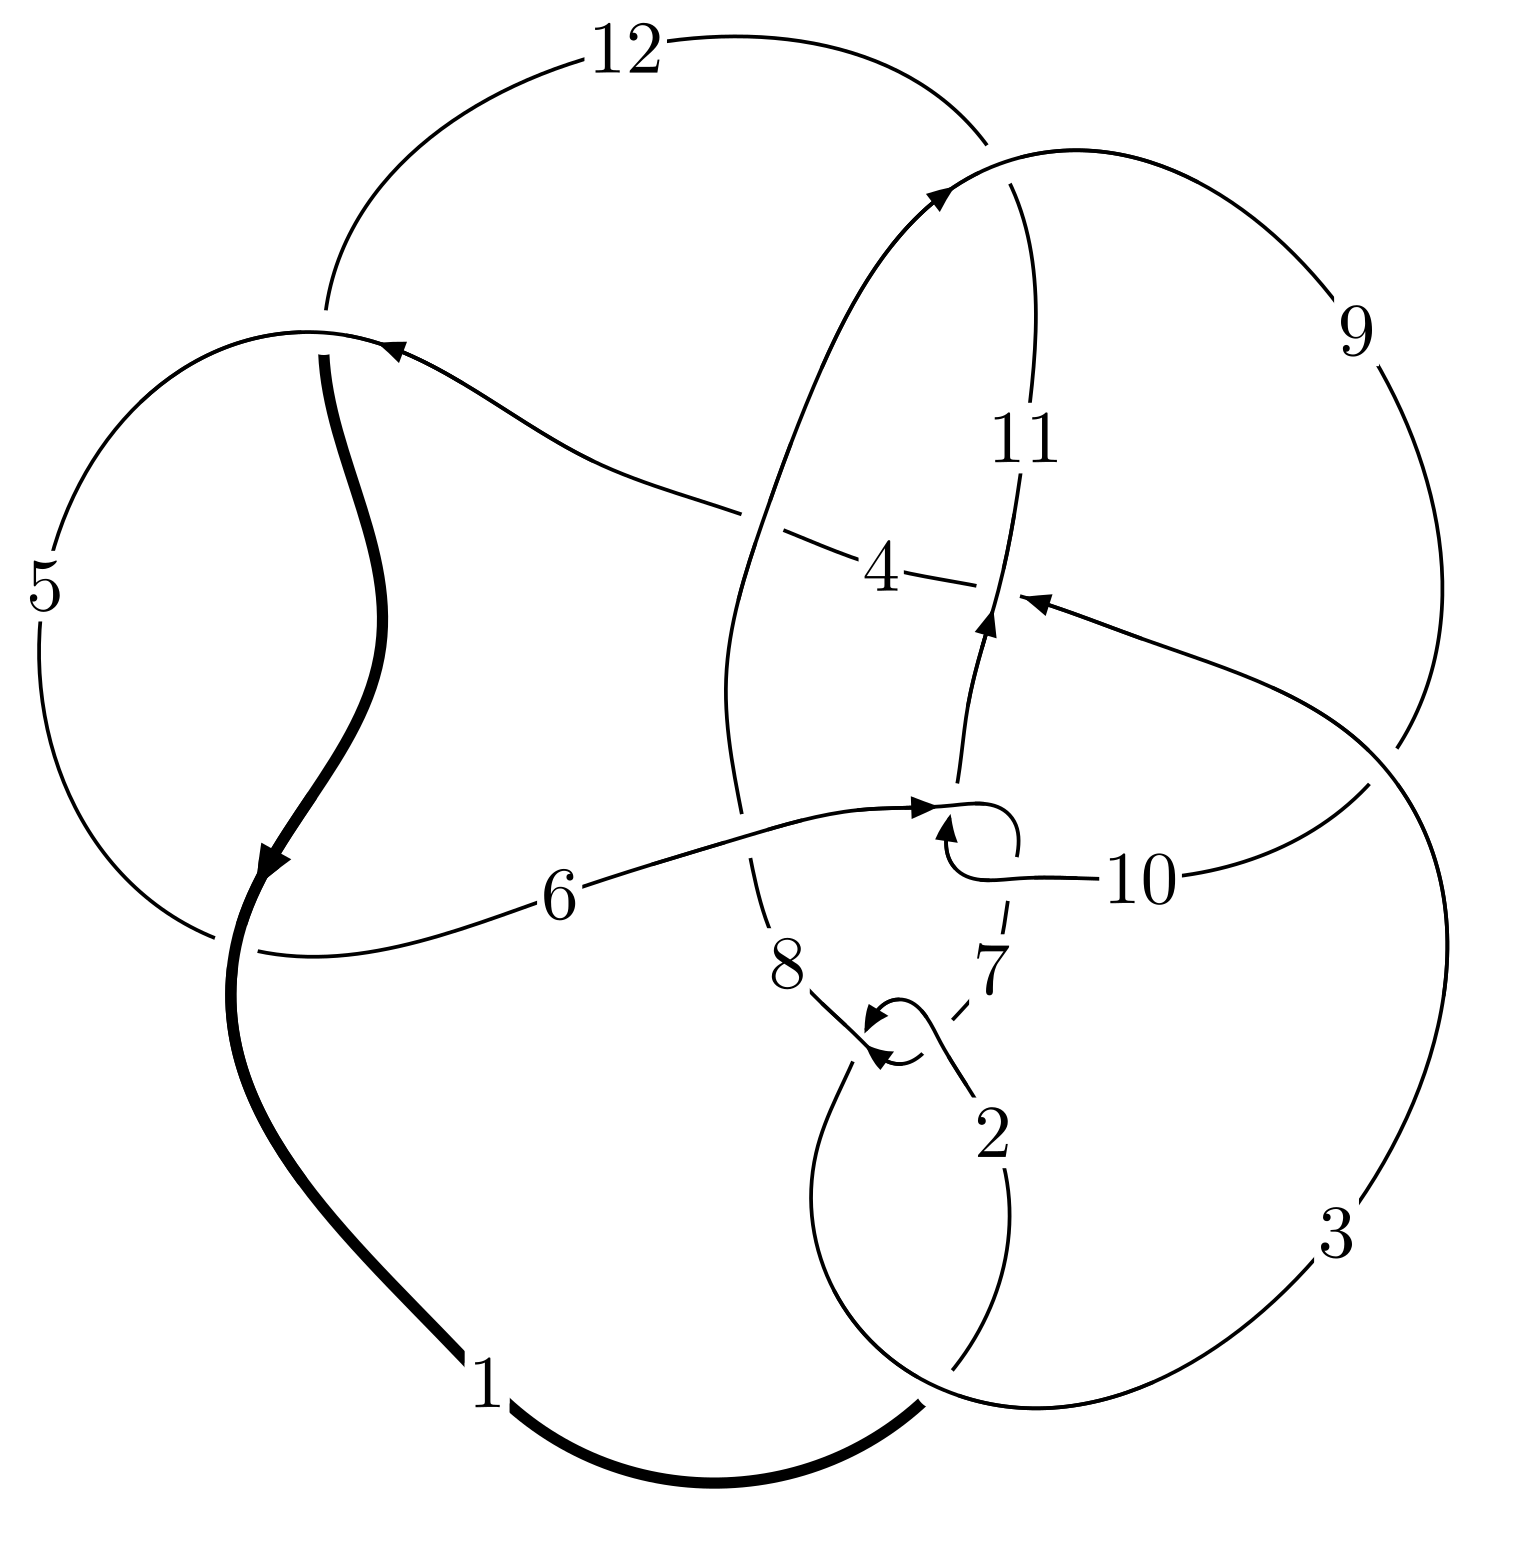
\includegraphics[width=112pt]{../../../GIT/diagram.site/Diagrams/png/2736_12n_0647.png}\\
\ \ \ A knot diagram\footnotemark}&
\allowdisplaybreaks
\textbf{Linearized knot diagam} \\
\cline{2-2}
 &
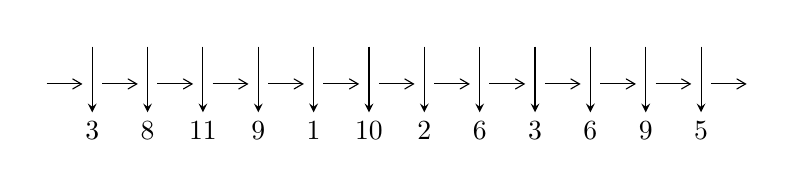
\begin{tikzpicture}[x=20pt, y=17pt]
	% nodes
	\node (C0) at (0, 0) {};
	\node (C1) at (1, 0) {};
	\node (C1U) at (1, +1) {};
	\node (C1D) at (1, -1) {3};

	\node (C2) at (2, 0) {};
	\node (C2U) at (2, +1) {};
	\node (C2D) at (2, -1) {8};

	\node (C3) at (3, 0) {};
	\node (C3U) at (3, +1) {};
	\node (C3D) at (3, -1) {11};

	\node (C4) at (4, 0) {};
	\node (C4U) at (4, +1) {};
	\node (C4D) at (4, -1) {9};

	\node (C5) at (5, 0) {};
	\node (C5U) at (5, +1) {};
	\node (C5D) at (5, -1) {1};

	\node (C6) at (6, 0) {};
	\node (C6U) at (6, +1) {};
	\node (C6D) at (6, -1) {10};

	\node (C7) at (7, 0) {};
	\node (C7U) at (7, +1) {};
	\node (C7D) at (7, -1) {2};

	\node (C8) at (8, 0) {};
	\node (C8U) at (8, +1) {};
	\node (C8D) at (8, -1) {6};

	\node (C9) at (9, 0) {};
	\node (C9U) at (9, +1) {};
	\node (C9D) at (9, -1) {3};

	\node (C10) at (10, 0) {};
	\node (C10U) at (10, +1) {};
	\node (C10D) at (10, -1) {6};

	\node (C11) at (11, 0) {};
	\node (C11U) at (11, +1) {};
	\node (C11D) at (11, -1) {9};

	\node (C12) at (12, 0) {};
	\node (C12U) at (12, +1) {};
	\node (C12D) at (12, -1) {5};
	\node (C13) at (13, 0) {};

	% arrows
	\draw[->,>={angle 60}]
	(C0) edge (C1) (C1) edge (C2) (C2) edge (C3) (C3) edge (C4) (C4) edge (C5) (C5) edge (C6) (C6) edge (C7) (C7) edge (C8) (C8) edge (C9) (C9) edge (C10) (C10) edge (C11) (C11) edge (C12) (C12) edge (C13) ;	\draw[->,>=stealth]
	(C1U) edge (C1D) (C2U) edge (C2D) (C3U) edge (C3D) (C4U) edge (C4D) (C5U) edge (C5D) (C6U) edge (C6D) (C7U) edge (C7D) (C8U) edge (C8D) (C9U) edge (C9D) (C10U) edge (C10D) (C11U) edge (C11D) (C12U) edge (C12D) ;
	\end{tikzpicture} \\
\hhline{~~} \\& 
\textbf{Solving Sequence} \\ \cline{2-2} 
 &
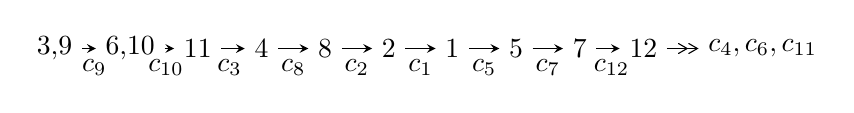
\begin{tikzpicture}[x=23pt, y=7pt]
	% node
	\node (A0) at (-1/8, 0) {3,9};
	\node (A1) at (17/16, 0) {6,10};
	\node (A2) at (17/8, 0) {11};
	\node (A3) at (25/8, 0) {4};
	\node (A4) at (33/8, 0) {8};
	\node (A5) at (41/8, 0) {2};
	\node (A6) at (49/8, 0) {1};
	\node (A7) at (57/8, 0) {5};
	\node (A8) at (65/8, 0) {7};
	\node (A9) at (73/8, 0) {12};
	\node (C1) at (1/2, -1) {$c_{9}$};
	\node (C2) at (13/8, -1) {$c_{10}$};
	\node (C3) at (21/8, -1) {$c_{3}$};
	\node (C4) at (29/8, -1) {$c_{8}$};
	\node (C5) at (37/8, -1) {$c_{2}$};
	\node (C6) at (45/8, -1) {$c_{1}$};
	\node (C7) at (53/8, -1) {$c_{5}$};
	\node (C8) at (61/8, -1) {$c_{7}$};
	\node (C9) at (69/8, -1) {$c_{12}$};
	\node (A10) at (11, 0) {$c_{4},c_{6},c_{11}$};

	% edge
	\draw[->,>=stealth]	
	(A0) edge (A1) (A1) edge (A2) (A2) edge (A3) (A3) edge (A4) (A4) edge (A5) (A5) edge (A6) (A6) edge (A7) (A7) edge (A8) (A8) edge (A9) ;
	\draw[->>,>={angle 60}]	
	(A9) edge (A10);
\end{tikzpicture} \\ 

\end{tabular} \\

\footnotetext{
The image of knot diagram is generated by the software ``\textbf{Draw programme}" developed by Andrew Bartholomew(\url{http://www.layer8.co.uk/maths/draw/index.htm\#Running-draw}), where we modified some parts for our purpose(\url{https://github.com/CATsTAILs/LinksPainter}).
}\phantom \\ \newline 
\centering \textbf{Ideals for irreducible components\footnotemark of $X_{\text{par}}$} 
 
\begin{align*}
I^u_{1}&=\langle 
-1.15739\times10^{38} u^{21}+2.59794\times10^{38} u^{20}+\cdots+5.63971\times10^{39} b+2.94029\times10^{39},\\
\phantom{I^u_{1}}&\phantom{= \langle  }1.52370\times10^{39} u^{21}-3.15147\times10^{38} u^{20}+\cdots+5.63971\times10^{39} a+6.37897\times10^{40},\;u^{22}- u^{21}+\cdots-7 u+1\rangle \\
I^u_{2}&=\langle 
2 u^{10}-2 u^9+3 u^8-5 u^7- u^6-3 u^5-5 u^4+8 u^3-6 u^2+b+8 u-1,\\
\phantom{I^u_{2}}&\phantom{= \langle  }u^{10}- u^9- u^7- u^6+u^5-2 u^4+3 u^3+a- u+2,\;u^{11}- u^8-3 u^7- u^6-3 u^5+2 u^4+2 u^3+3 u-1\rangle \\
\\
\end{align*}
\raggedright * 2 irreducible components of $\dim_{\mathbb{C}}=0$, with total 33 representations.\\
\footnotetext{All coefficients of polynomials are rational numbers. But the coefficients are sometimes approximated in decimal forms when there is not enough margin.}
\newpage
\renewcommand{\arraystretch}{1}
\centering \section*{I. $I^u_{1}= \langle -1.16\times10^{38} u^{21}+2.60\times10^{38} u^{20}+\cdots+5.64\times10^{39} b+2.94\times10^{39},\;1.52\times10^{39} u^{21}-3.15\times10^{38} u^{20}+\cdots+5.64\times10^{39} a+6.38\times10^{40},\;u^{22}- u^{21}+\cdots-7 u+1 \rangle$}
\flushleft \textbf{(i) Arc colorings}\\
\begin{tabular}{m{7pt} m{180pt} m{7pt} m{180pt} }
\flushright $a_{3}=$&$\begin{pmatrix}0\\u\end{pmatrix}$ \\
\flushright $a_{9}=$&$\begin{pmatrix}1\\0\end{pmatrix}$ \\
\flushright $a_{6}=$&$\begin{pmatrix}-0.270174 u^{21}+0.0558800 u^{20}+\cdots+42.5373 u-11.3108\\0.0205221 u^{21}-0.0460651 u^{20}+\cdots+6.82322 u-0.521354\end{pmatrix}$ \\
\flushright $a_{10}=$&$\begin{pmatrix}1\\u^2\end{pmatrix}$ \\
\flushright $a_{11}=$&$\begin{pmatrix}-1.35047 u^{21}+1.35347 u^{20}+\cdots-117.421 u+7.69784\\-0.209846 u^{21}+0.147595 u^{20}+\cdots-6.54594 u+0.116749\end{pmatrix}$ \\
\flushright $a_{4}=$&$\begin{pmatrix}2.15834 u^{21}-2.04296 u^{20}+\cdots+162.698 u-7.98991\\0.318765 u^{21}-0.225148 u^{20}+\cdots+8.95792 u-0.0968802\end{pmatrix}$ \\
\flushright $a_{8}=$&$\begin{pmatrix}1.18213 u^{21}-1.17546 u^{20}+\cdots+97.8267 u-4.07571\\0.214154 u^{21}-0.137619 u^{20}+\cdots+5.41053 u-0.123423\end{pmatrix}$ \\
\flushright $a_{2}=$&$\begin{pmatrix}-1.66406 u^{21}+1.47272 u^{20}+\cdots-96.5661 u-0.246377\\-0.256597 u^{21}+0.176966 u^{20}+\cdots-3.09765 u+0.0237528\end{pmatrix}$ \\
\flushright $a_{1}=$&$\begin{pmatrix}-1.66406 u^{21}+1.47272 u^{20}+\cdots-96.5661 u-0.246377\\-0.227217 u^{21}+0.158707 u^{20}+\cdots-3.42237 u-0.167580\end{pmatrix}$ \\
\flushright $a_{5}=$&$\begin{pmatrix}1.83958 u^{21}-1.81781 u^{20}+\cdots+153.740 u-7.89303\\0.318765 u^{21}-0.225148 u^{20}+\cdots+8.95792 u-0.0968802\end{pmatrix}$ \\
\flushright $a_{7}=$&$\begin{pmatrix}-0.297455 u^{21}+0.112963 u^{20}+\cdots+34.4842 u-10.5752\\0.0338753 u^{21}-0.0534463 u^{20}+\cdots+7.05911 u-0.551156\end{pmatrix}$ \\
\flushright $a_{12}=$&$\begin{pmatrix}1.14063 u^{21}-1.20587 u^{20}+\cdots+110.875 u-7.58109\\0.209846 u^{21}-0.147595 u^{20}+\cdots+6.54594 u-0.116749\end{pmatrix}$\\&\end{tabular}
\flushleft \textbf{(ii) Obstruction class $= -1$}\\~\\
\flushleft \textbf{(iii) Cusp Shapes $= -1.01325 u^{21}+1.04755 u^{20}+\cdots-80.2731 u-9.63814$}\\~\\
\newpage\renewcommand{\arraystretch}{1}
\flushleft \textbf{(iv) u-Polynomials at the component}\newline \\
\begin{tabular}{m{50pt}|m{274pt}}
Crossings & \hspace{64pt}u-Polynomials at each crossing \\
\hline $$\begin{aligned}c_{1}\end{aligned}$$&$\begin{aligned}
&u^{22}+9 u^{21}+\cdots+637 u+49
\end{aligned}$\\
\hline $$\begin{aligned}c_{2},c_{7}\end{aligned}$$&$\begin{aligned}
&u^{22}+u^{21}+\cdots-35 u-7
\end{aligned}$\\
\hline $$\begin{aligned}c_{3},c_{5},c_{12}\end{aligned}$$&$\begin{aligned}
&u^{22}+2 u^{21}+\cdots- u+1
\end{aligned}$\\
\hline $$\begin{aligned}c_{4}\end{aligned}$$&$\begin{aligned}
&u^{22}+2 u^{21}+\cdots-5 u+1
\end{aligned}$\\
\hline $$\begin{aligned}c_{6},c_{10}\end{aligned}$$&$\begin{aligned}
&u^{22}+2 u^{21}+\cdots-66 u-19
\end{aligned}$\\
\hline $$\begin{aligned}c_{8}\end{aligned}$$&$\begin{aligned}
&u^{22}-3 u^{21}+\cdots+85 u+23
\end{aligned}$\\
\hline $$\begin{aligned}c_{9}\end{aligned}$$&$\begin{aligned}
&u^{22}- u^{21}+\cdots-7 u+1
\end{aligned}$\\
\hline $$\begin{aligned}c_{11}\end{aligned}$$&$\begin{aligned}
&u^{22}-6 u^{21}+\cdots-2 u+1
\end{aligned}$\\
\hline
\end{tabular}\\~\\
\newpage\renewcommand{\arraystretch}{1}
\flushleft \textbf{(v) Riley Polynomials at the component}\newline \\
\begin{tabular}{m{50pt}|m{274pt}}
Crossings & \hspace{64pt}Riley Polynomials at each crossing \\
\hline $$\begin{aligned}c_{1}\end{aligned}$$&$\begin{aligned}
&y^{22}+19 y^{21}+\cdots-134113 y+2401
\end{aligned}$\\
\hline $$\begin{aligned}c_{2},c_{7}\end{aligned}$$&$\begin{aligned}
&y^{22}-9 y^{21}+\cdots-637 y+49
\end{aligned}$\\
\hline $$\begin{aligned}c_{3},c_{5},c_{12}\end{aligned}$$&$\begin{aligned}
&y^{22}-20 y^{21}+\cdots-85 y+1
\end{aligned}$\\
\hline $$\begin{aligned}c_{4}\end{aligned}$$&$\begin{aligned}
&y^{22}-40 y^{21}+\cdots-25 y+1
\end{aligned}$\\
\hline $$\begin{aligned}c_{6},c_{10}\end{aligned}$$&$\begin{aligned}
&y^{22}+24 y^{21}+\cdots-4660 y+361
\end{aligned}$\\
\hline $$\begin{aligned}c_{8}\end{aligned}$$&$\begin{aligned}
&y^{22}+29 y^{21}+\cdots-9065 y+529
\end{aligned}$\\
\hline $$\begin{aligned}c_{9}\end{aligned}$$&$\begin{aligned}
&y^{22}+39 y^{21}+\cdots+117 y+1
\end{aligned}$\\
\hline $$\begin{aligned}c_{11}\end{aligned}$$&$\begin{aligned}
&y^{22}-52 y^{21}+\cdots-36 y+1
\end{aligned}$\\
\hline
\end{tabular}\\~\\
\newpage\flushleft \textbf{(vi) Complex Volumes and Cusp Shapes}
$$\begin{array}{c|c|c}  
\text{Solutions to }I^u_{1}& \I (\text{vol} + \sqrt{-1}CS) & \text{Cusp shape}\\
 \hline 
\begin{aligned}
u &= \phantom{-}0.922193 + 0.451969 I \\
a &= -0.140167 + 0.079897 I \\
b &= -1.135600 + 0.625368 I\end{aligned}
 & -3.68279 - 0.94185 I & -15.4912 + 3.1680 I \\ \hline\begin{aligned}
u &= \phantom{-}0.922193 - 0.451969 I \\
a &= -0.140167 - 0.079897 I \\
b &= -1.135600 - 0.625368 I\end{aligned}
 & -3.68279 + 0.94185 I & -15.4912 - 3.1680 I \\ \hline\begin{aligned}
u &= -0.918387 + 0.590013 I \\
a &= \phantom{-}0.823390 + 0.318747 I \\
b &= \phantom{-}0.795349 + 0.331962 I\end{aligned}
 & -0.88400 - 1.53763 I & -11.84759 + 1.75542 I \\ \hline\begin{aligned}
u &= -0.918387 - 0.590013 I \\
a &= \phantom{-}0.823390 - 0.318747 I \\
b &= \phantom{-}0.795349 - 0.331962 I\end{aligned}
 & -0.88400 + 1.53763 I & -11.84759 - 1.75542 I \\ \hline\begin{aligned}
u &= -0.015535 + 1.113510 I \\
a &= \phantom{-}0.50175 + 1.35452 I \\
b &= -0.093079 - 0.699578 I\end{aligned}
 & -1.24345 - 2.09162 I & -12.32634 + 3.76479 I \\ \hline\begin{aligned}
u &= -0.015535 - 1.113510 I \\
a &= \phantom{-}0.50175 - 1.35452 I \\
b &= -0.093079 + 0.699578 I\end{aligned}
 & -1.24345 + 2.09162 I & -12.32634 - 3.76479 I \\ \hline\begin{aligned}
u &= \phantom{-}1.14626\phantom{ +0.000000I} \\
a &= -0.626888\phantom{ +0.000000I} \\
b &= \phantom{-}0.600846\phantom{ +0.000000I}\end{aligned}
 & -7.73402\phantom{ +0.000000I} & -2.06680\phantom{ +0.000000I} \\ \hline\begin{aligned}
u &= \phantom{-}0.40719 + 1.44071 I \\
a &= \phantom{-}0.364074 - 0.930543 I \\
b &= -0.38730 + 1.37848 I\end{aligned}
 & \phantom{-}1.70191 + 1.70598 I & -14.8255 - 1.4132 I \\ \hline\begin{aligned}
u &= \phantom{-}0.40719 - 1.44071 I \\
a &= \phantom{-}0.364074 + 0.930543 I \\
b &= -0.38730 - 1.37848 I\end{aligned}
 & \phantom{-}1.70191 - 1.70598 I & -14.8255 + 1.4132 I \\ \hline\begin{aligned}
u &= \phantom{-}0.317847 + 0.269046 I \\
a &= \phantom{-}2.62385 - 0.79046 I \\
b &= -0.085195 + 0.903480 I\end{aligned}
 & \phantom{-}1.56638 + 2.34323 I & -10.66731 - 5.68174 I\\
 \hline 
 \end{array}$$\newpage$$\begin{array}{c|c|c}  
\text{Solutions to }I^u_{1}& \I (\text{vol} + \sqrt{-1}CS) & \text{Cusp shape}\\
 \hline 
\begin{aligned}
u &= \phantom{-}0.317847 - 0.269046 I \\
a &= \phantom{-}2.62385 + 0.79046 I \\
b &= -0.085195 - 0.903480 I\end{aligned}
 & \phantom{-}1.56638 - 2.34323 I & -10.66731 + 5.68174 I \\ \hline\begin{aligned}
u &= \phantom{-}0.403521\phantom{ +0.000000I} \\
a &= \phantom{-}2.31915\phantom{ +0.000000I} \\
b &= \phantom{-}1.67477\phantom{ +0.000000I}\end{aligned}
 & -13.6204\phantom{ +0.000000I} & -17.7340\phantom{ +0.000000I} \\ \hline\begin{aligned}
u &= -0.352636\phantom{ +0.000000I} \\
a &= \phantom{-}0.655926\phantom{ +0.000000I} \\
b &= -0.220728\phantom{ +0.000000I}\end{aligned}
 & -0.550682\phantom{ +0.000000I} & -18.1690\phantom{ +0.000000I} \\ \hline\begin{aligned}
u &= -1.87169\phantom{ +0.000000I} \\
a &= -0.326736\phantom{ +0.000000I} \\
b &= -0.803005\phantom{ +0.000000I}\end{aligned}
 & -14.8041\phantom{ +0.000000I} & -12.3900\phantom{ +0.000000I} \\ \hline\begin{aligned}
u &= \phantom{-}0.0195375 + 0.1177480 I \\
a &= -10.81320 + 5.82406 I \\
b &= -0.225273 + 0.760617 I\end{aligned}
 & -3.29787 + 5.70936 I & -15.2173 - 7.8009 I \\ \hline\begin{aligned}
u &= \phantom{-}0.0195375 - 0.1177480 I \\
a &= -10.81320 - 5.82406 I \\
b &= -0.225273 - 0.760617 I\end{aligned}
 & -3.29787 - 5.70936 I & -15.2173 + 7.8009 I \\ \hline\begin{aligned}
u &= \phantom{-}0.78622 + 2.42733 I \\
a &= \phantom{-}0.107388 - 0.674968 I \\
b &= \phantom{-}0.95174 + 2.08123 I\end{aligned}
 & \phantom{-}5.54115 - 10.77480 I & \phantom{-0.000000 } 0 \\ \hline\begin{aligned}
u &= \phantom{-}0.78622 - 2.42733 I \\
a &= \phantom{-}0.107388 + 0.674968 I \\
b &= \phantom{-}0.95174 - 2.08123 I\end{aligned}
 & \phantom{-}5.54115 + 10.77480 I & \phantom{-0.000000 } 0 \\ \hline\begin{aligned}
u &= -0.24073 + 2.68361 I \\
a &= -0.036423 - 0.623368 I \\
b &= \phantom{-}0.27638 + 2.41167 I\end{aligned}
 & \phantom{-}8.25134 + 2.56104 I & \phantom{-0.000000 } 0 \\ \hline\begin{aligned}
u &= -0.24073 - 2.68361 I \\
a &= -0.036423 + 0.623368 I \\
b &= \phantom{-}0.27638 - 2.41167 I\end{aligned}
 & \phantom{-}8.25134 - 2.56104 I & \phantom{-0.000000 } 0\\
 \hline 
 \end{array}$$\newpage$$\begin{array}{c|c|c}  
\text{Solutions to }I^u_{1}& \I (\text{vol} + \sqrt{-1}CS) & \text{Cusp shape}\\
 \hline 
\begin{aligned}
u &= -0.44105 + 2.79932 I \\
a &= \phantom{-}0.058592 + 0.603776 I \\
b &= \phantom{-}0.77704 - 2.39189 I\end{aligned}
 & \phantom{-}11.22440 + 4.41241 I & \phantom{-0.000000 } 0 \\ \hline\begin{aligned}
u &= -0.44105 - 2.79932 I \\
a &= \phantom{-}0.058592 - 0.603776 I \\
b &= \phantom{-}0.77704 + 2.39189 I\end{aligned}
 & \phantom{-}11.22440 - 4.41241 I & \phantom{-0.000000 } 0\\
 \hline 
 \end{array}$$\newpage\newpage\renewcommand{\arraystretch}{1}
\centering \section*{II. $I^u_{2}= \langle 2 u^{10}-2 u^9+\cdots+b-1,\;u^{10}- u^9- u^7- u^6+u^5-2 u^4+3 u^3+a- u+2,\;u^{11}- u^8-3 u^7- u^6-3 u^5+2 u^4+2 u^3+3 u-1 \rangle$}
\flushleft \textbf{(i) Arc colorings}\\
\begin{tabular}{m{7pt} m{180pt} m{7pt} m{180pt} }
\flushright $a_{3}=$&$\begin{pmatrix}0\\u\end{pmatrix}$ \\
\flushright $a_{9}=$&$\begin{pmatrix}1\\0\end{pmatrix}$ \\
\flushright $a_{6}=$&$\begin{pmatrix}- u^{10}+u^9+u^7+u^6- u^5+2 u^4-3 u^3+u-2\\-2 u^{10}+2 u^9-3 u^8+5 u^7+u^6+3 u^5+5 u^4-8 u^3+6 u^2-8 u+1\end{pmatrix}$ \\
\flushright $a_{10}=$&$\begin{pmatrix}1\\u^2\end{pmatrix}$ \\
\flushright $a_{11}=$&$\begin{pmatrix}2 u^{10}- u^9+u^8-3 u^7-3 u^6-2 u^5-5 u^4+5 u^3- u^2+2 u+2\\u^2+1\end{pmatrix}$ \\
\flushright $a_{4}=$&$\begin{pmatrix}u^{10}-2 u^9+3 u^8-4 u^7+2 u^6-2 u^5-2 u^4+6 u^3-8 u^2+8 u-4\\2 u^{10}-3 u^9+3 u^8-6 u^7+u^6- u^5-3 u^4+11 u^3-7 u^2+9 u-3\end{pmatrix}$ \\
\flushright $a_{8}=$&$\begin{pmatrix}-2 u^{10}+2 u^9-2 u^8+4 u^7+u^6+u^5+5 u^4-7 u^3+5 u^2-4 u\\-2 u^{10}+2 u^9-3 u^8+5 u^7+u^6+3 u^5+5 u^4-8 u^3+5 u^2-8 u+1\end{pmatrix}$ \\
\flushright $a_{2}=$&$\begin{pmatrix}u^{10}-2 u^9+2 u^8-3 u^7+u^6-2 u^4+7 u^3-5 u^2+5 u-1\\-2 u^{10}+3 u^9-3 u^8+5 u^7- u^6+u^5+4 u^4-10 u^3+8 u^2-6 u+2\end{pmatrix}$ \\
\flushright $a_{1}=$&$\begin{pmatrix}u^{10}-2 u^9+2 u^8-3 u^7+u^6-2 u^4+7 u^3-5 u^2+5 u-1\\-4 u^{10}+5 u^9-5 u^8+10 u^7+2 u^5+7 u^4-19 u^3+12 u^2-13 u+4\end{pmatrix}$ \\
\flushright $a_{5}=$&$\begin{pmatrix}- u^{10}+u^9+2 u^7+u^6- u^5+u^4-5 u^3- u^2- u-1\\2 u^{10}-3 u^9+3 u^8-6 u^7+u^6- u^5-3 u^4+11 u^3-7 u^2+9 u-3\end{pmatrix}$ \\
\flushright $a_{7}=$&$\begin{pmatrix}u^{10}- u^9+2 u^8-3 u^7-2 u^5-3 u^4+4 u^3-5 u^2+5 u-2\\-1\end{pmatrix}$ \\
\flushright $a_{12}=$&$\begin{pmatrix}2 u^{10}- u^9+u^8-3 u^7-3 u^6-2 u^5-5 u^4+5 u^3-2 u^2+2 u+1\\u^2+1\end{pmatrix}$\\&\end{tabular}
\flushleft \textbf{(ii) Obstruction class $= 1$}\\~\\
\flushleft \textbf{(iii) Cusp Shapes $= 18 u^{10}-18 u^9+22 u^8-45 u^7-8 u^6-17 u^5-37 u^4+76 u^3-49 u^2+62 u-28$}\\~\\
\newpage\renewcommand{\arraystretch}{1}
\flushleft \textbf{(iv) u-Polynomials at the component}\newline \\
\begin{tabular}{m{50pt}|m{274pt}}
Crossings & \hspace{64pt}u-Polynomials at each crossing \\
\hline $$\begin{aligned}c_{1}\end{aligned}$$&$\begin{aligned}
&u^{11}-12 u^{10}+\cdots+19 u-1
\end{aligned}$\\
\hline $$\begin{aligned}c_{2}\end{aligned}$$&$\begin{aligned}
&u^{11}-6 u^9+u^8+14 u^7-4 u^6-17 u^5+6 u^4+11 u^3-5 u^2-3 u+1
\end{aligned}$\\
\hline $$\begin{aligned}c_{3},c_{5}\end{aligned}$$&$\begin{aligned}
&u^{11}- u^{10}-7 u^9+6 u^8+18 u^7-12 u^6-20 u^5+8 u^4+7 u^3+u^2+u-1
\end{aligned}$\\
\hline $$\begin{aligned}c_{4}\end{aligned}$$&$\begin{aligned}
&u^{11}+u^{10}+\cdots+7 u-1
\end{aligned}$\\
\hline $$\begin{aligned}c_{6}\end{aligned}$$&$\begin{aligned}
&u^{11}+u^{10}- u^9+2 u^8-2 u^6+3 u^5-3 u^4+u^2-2 u+1
\end{aligned}$\\
\hline $$\begin{aligned}c_{7}\end{aligned}$$&$\begin{aligned}
&u^{11}-6 u^9- u^8+14 u^7+4 u^6-17 u^5-6 u^4+11 u^3+5 u^2-3 u-1
\end{aligned}$\\
\hline $$\begin{aligned}c_{8}\end{aligned}$$&$\begin{aligned}
&u^{11}+2 u^{10}+u^9-3 u^7-3 u^6-2 u^5+2 u^3+u^2+u-1
\end{aligned}$\\
\hline $$\begin{aligned}c_{9}\end{aligned}$$&$\begin{aligned}
&u^{11}- u^8-3 u^7- u^6-3 u^5+2 u^4+2 u^3+3 u-1
\end{aligned}$\\
\hline $$\begin{aligned}c_{10}\end{aligned}$$&$\begin{aligned}
&u^{11}- u^{10}- u^9-2 u^8+2 u^6+3 u^5+3 u^4- u^2-2 u-1
\end{aligned}$\\
\hline $$\begin{aligned}c_{11}\end{aligned}$$&$\begin{aligned}
&u^{11}+11 u^{10}+\cdots+6 u+1
\end{aligned}$\\
\hline $$\begin{aligned}c_{12}\end{aligned}$$&$\begin{aligned}
&u^{11}+u^{10}-7 u^9-6 u^8+18 u^7+12 u^6-20 u^5-8 u^4+7 u^3- u^2+u+1
\end{aligned}$\\
\hline
\end{tabular}\\~\\
\newpage\renewcommand{\arraystretch}{1}
\flushleft \textbf{(v) Riley Polynomials at the component}\newline \\
\begin{tabular}{m{50pt}|m{274pt}}
Crossings & \hspace{64pt}Riley Polynomials at each crossing \\
\hline $$\begin{aligned}c_{1}\end{aligned}$$&$\begin{aligned}
&y^{11}-16 y^{10}+\cdots+155 y-1
\end{aligned}$\\
\hline $$\begin{aligned}c_{2},c_{7}\end{aligned}$$&$\begin{aligned}
&y^{11}-12 y^{10}+\cdots+19 y-1
\end{aligned}$\\
\hline $$\begin{aligned}c_{3},c_{5},c_{12}\end{aligned}$$&$\begin{aligned}
&y^{11}-15 y^{10}+\cdots+3 y-1
\end{aligned}$\\
\hline $$\begin{aligned}c_{4}\end{aligned}$$&$\begin{aligned}
&y^{11}-31 y^{10}+\cdots+15 y-1
\end{aligned}$\\
\hline $$\begin{aligned}c_{6},c_{10}\end{aligned}$$&$\begin{aligned}
&y^{11}-3 y^{10}-3 y^9+6 y^8+8 y^7+2 y^6-5 y^5-9 y^4-2 y^3+5 y^2+2 y-1
\end{aligned}$\\
\hline $$\begin{aligned}c_{8}\end{aligned}$$&$\begin{aligned}
&y^{11}-2 y^{10}-5 y^9+2 y^8+9 y^7+5 y^6-2 y^5-8 y^4-6 y^3+3 y^2+3 y-1
\end{aligned}$\\
\hline $$\begin{aligned}c_{9}\end{aligned}$$&$\begin{aligned}
&y^{11}-6 y^9-7 y^8+11 y^7+27 y^6+y^5-36 y^4-16 y^3+16 y^2+9 y-1
\end{aligned}$\\
\hline $$\begin{aligned}c_{11}\end{aligned}$$&$\begin{aligned}
&y^{11}-23 y^{10}+\cdots-10 y-1
\end{aligned}$\\
\hline
\end{tabular}\\~\\
\newpage\flushleft \textbf{(vi) Complex Volumes and Cusp Shapes}
$$\begin{array}{c|c|c}  
\text{Solutions to }I^u_{2}& \I (\text{vol} + \sqrt{-1}CS) & \text{Cusp shape}\\
 \hline 
\begin{aligned}
u &= \phantom{-}0.946698\phantom{ +0.000000I} \\
a &= -1.31867\phantom{ +0.000000I} \\
b &= \phantom{-}0.570624\phantom{ +0.000000I}\end{aligned}
 & -10.8918\phantom{ +0.000000I} & -14.2030\phantom{ +0.000000I} \\ \hline\begin{aligned}
u &= \phantom{-}0.107517 + 0.921326 I \\
a &= -0.41829 + 1.75925 I \\
b &= -0.627508 - 0.776878 I\end{aligned}
 & -1.39916 + 0.85773 I & -12.76968 + 1.45970 I \\ \hline\begin{aligned}
u &= \phantom{-}0.107517 - 0.921326 I \\
a &= -0.41829 - 1.75925 I \\
b &= -0.627508 + 0.776878 I\end{aligned}
 & -1.39916 - 0.85773 I & -12.76968 - 1.45970 I \\ \hline\begin{aligned}
u &= -1.13392\phantom{ +0.000000I} \\
a &= -0.477082\phantom{ +0.000000I} \\
b &= \phantom{-}0.739267\phantom{ +0.000000I}\end{aligned}
 & -8.01807\phantom{ +0.000000I} & -30.7780\phantom{ +0.000000I} \\ \hline\begin{aligned}
u &= -1.14734\phantom{ +0.000000I} \\
a &= -0.896870\phantom{ +0.000000I} \\
b &= -1.75156\phantom{ +0.000000I}\end{aligned}
 & -12.5057\phantom{ +0.000000I} & -9.97480\phantom{ +0.000000I} \\ \hline\begin{aligned}
u &= \phantom{-}0.206612 + 1.130010 I \\
a &= \phantom{-}0.53803 - 1.36462 I \\
b &= -0.270708 + 1.018240 I\end{aligned}
 & \phantom{-}2.65235 + 1.78346 I & -4.71612 - 3.09744 I \\ \hline\begin{aligned}
u &= \phantom{-}0.206612 - 1.130010 I \\
a &= \phantom{-}0.53803 + 1.36462 I \\
b &= -0.270708 - 1.018240 I\end{aligned}
 & \phantom{-}2.65235 - 1.78346 I & -4.71612 + 3.09744 I \\ \hline\begin{aligned}
u &= -0.562339 + 1.094490 I \\
a &= \phantom{-}1.066280 + 0.765572 I \\
b &= \phantom{-}0.113141 - 1.003800 I\end{aligned}
 & -2.63212 - 4.42190 I & -12.78415 + 2.93693 I \\ \hline\begin{aligned}
u &= -0.562339 - 1.094490 I \\
a &= \phantom{-}1.066280 - 0.765572 I \\
b &= \phantom{-}0.113141 + 1.003800 I\end{aligned}
 & -2.63212 + 4.42190 I & -12.78415 - 2.93693 I \\ \hline\begin{aligned}
u &= \phantom{-}1.52035\phantom{ +0.000000I} \\
a &= \phantom{-}0.0829538\phantom{ +0.000000I} \\
b &= \phantom{-}1.10046\phantom{ +0.000000I}\end{aligned}
 & -15.4881\phantom{ +0.000000I} & -24.9010\phantom{ +0.000000I}\\
 \hline 
 \end{array}$$\newpage$$\begin{array}{c|c|c}  
\text{Solutions to }I^u_{2}& \I (\text{vol} + \sqrt{-1}CS) & \text{Cusp shape}\\
 \hline 
\begin{aligned}
u &= \phantom{-}0.310641\phantom{ +0.000000I} \\
a &= -1.76236\phantom{ +0.000000I} \\
b &= -1.08864\phantom{ +0.000000I}\end{aligned}
 & -2.97640\phantom{ +0.000000I} & -11.6020\phantom{ +0.000000I}\\
 \hline 
 \end{array}$$\newpage
\newpage\renewcommand{\arraystretch}{1}
\centering \section*{ III. u-Polynomials}
\begin{tabular}{m{50pt}|m{274pt}}
Crossings & \hspace{64pt}u-Polynomials at each crossing \\
\hline $$\begin{aligned}c_{1}\end{aligned}$$&$\begin{aligned}
&(u^{11}-12 u^{10}+\cdots+19 u-1)(u^{22}+9 u^{21}+\cdots+637 u+49)
\end{aligned}$\\
\hline $$\begin{aligned}c_{2}\end{aligned}$$&$\begin{aligned}
&(u^{11}-6 u^9+u^8+14 u^7-4 u^6-17 u^5+6 u^4+11 u^3-5 u^2-3 u+1)\\
&\cdot(u^{22}+u^{21}+\cdots-35 u-7)
\end{aligned}$\\
\hline $$\begin{aligned}c_{3},c_{5}\end{aligned}$$&$\begin{aligned}
&(u^{11}- u^{10}-7 u^9+6 u^8+18 u^7-12 u^6-20 u^5+8 u^4+7 u^3+u^2+u-1)\\
&\cdot(u^{22}+2 u^{21}+\cdots- u+1)
\end{aligned}$\\
\hline $$\begin{aligned}c_{4}\end{aligned}$$&$\begin{aligned}
&(u^{11}+u^{10}+\cdots+7 u-1)(u^{22}+2 u^{21}+\cdots-5 u+1)
\end{aligned}$\\
\hline $$\begin{aligned}c_{6}\end{aligned}$$&$\begin{aligned}
&(u^{11}+u^{10}- u^9+2 u^8-2 u^6+3 u^5-3 u^4+u^2-2 u+1)\\
&\cdot(u^{22}+2 u^{21}+\cdots-66 u-19)
\end{aligned}$\\
\hline $$\begin{aligned}c_{7}\end{aligned}$$&$\begin{aligned}
&(u^{11}-6 u^9- u^8+14 u^7+4 u^6-17 u^5-6 u^4+11 u^3+5 u^2-3 u-1)\\
&\cdot(u^{22}+u^{21}+\cdots-35 u-7)
\end{aligned}$\\
\hline $$\begin{aligned}c_{8}\end{aligned}$$&$\begin{aligned}
&(u^{11}+2 u^{10}+u^9-3 u^7-3 u^6-2 u^5+2 u^3+u^2+u-1)\\
&\cdot(u^{22}-3 u^{21}+\cdots+85 u+23)
\end{aligned}$\\
\hline $$\begin{aligned}c_{9}\end{aligned}$$&$\begin{aligned}
&(u^{11}- u^8+\cdots+3 u-1)(u^{22}- u^{21}+\cdots-7 u+1)
\end{aligned}$\\
\hline $$\begin{aligned}c_{10}\end{aligned}$$&$\begin{aligned}
&(u^{11}- u^{10}- u^9-2 u^8+2 u^6+3 u^5+3 u^4- u^2-2 u-1)\\
&\cdot(u^{22}+2 u^{21}+\cdots-66 u-19)
\end{aligned}$\\
\hline $$\begin{aligned}c_{11}\end{aligned}$$&$\begin{aligned}
&(u^{11}+11 u^{10}+\cdots+6 u+1)(u^{22}-6 u^{21}+\cdots-2 u+1)
\end{aligned}$\\
\hline $$\begin{aligned}c_{12}\end{aligned}$$&$\begin{aligned}
&(u^{11}+u^{10}-7 u^9-6 u^8+18 u^7+12 u^6-20 u^5-8 u^4+7 u^3- u^2+u+1)\\
&\cdot(u^{22}+2 u^{21}+\cdots- u+1)
\end{aligned}$\\
\hline
\end{tabular}\newpage\renewcommand{\arraystretch}{1}
\centering \section*{ IV. Riley Polynomials}
\begin{tabular}{m{50pt}|m{274pt}}
Crossings & \hspace{64pt}Riley Polynomials at each crossing \\
\hline $$\begin{aligned}c_{1}\end{aligned}$$&$\begin{aligned}
&(y^{11}-16 y^{10}+\cdots+155 y-1)(y^{22}+19 y^{21}+\cdots-134113 y+2401)
\end{aligned}$\\
\hline $$\begin{aligned}c_{2},c_{7}\end{aligned}$$&$\begin{aligned}
&(y^{11}-12 y^{10}+\cdots+19 y-1)(y^{22}-9 y^{21}+\cdots-637 y+49)
\end{aligned}$\\
\hline $$\begin{aligned}c_{3},c_{5},c_{12}\end{aligned}$$&$\begin{aligned}
&(y^{11}-15 y^{10}+\cdots+3 y-1)(y^{22}-20 y^{21}+\cdots-85 y+1)
\end{aligned}$\\
\hline $$\begin{aligned}c_{4}\end{aligned}$$&$\begin{aligned}
&(y^{11}-31 y^{10}+\cdots+15 y-1)(y^{22}-40 y^{21}+\cdots-25 y+1)
\end{aligned}$\\
\hline $$\begin{aligned}c_{6},c_{10}\end{aligned}$$&$\begin{aligned}
&(y^{11}-3 y^{10}-3 y^9+6 y^8+8 y^7+2 y^6-5 y^5-9 y^4-2 y^3+5 y^2+2 y-1)\\
&\cdot(y^{22}+24 y^{21}+\cdots-4660 y+361)
\end{aligned}$\\
\hline $$\begin{aligned}c_{8}\end{aligned}$$&$\begin{aligned}
&(y^{11}-2 y^{10}-5 y^9+2 y^8+9 y^7+5 y^6-2 y^5-8 y^4-6 y^3+3 y^2+3 y-1)\\
&\cdot(y^{22}+29 y^{21}+\cdots-9065 y+529)
\end{aligned}$\\
\hline $$\begin{aligned}c_{9}\end{aligned}$$&$\begin{aligned}
&(y^{11}-6 y^9-7 y^8+11 y^7+27 y^6+y^5-36 y^4-16 y^3+16 y^2+9 y-1)\\
&\cdot(y^{22}+39 y^{21}+\cdots+117 y+1)
\end{aligned}$\\
\hline $$\begin{aligned}c_{11}\end{aligned}$$&$\begin{aligned}
&(y^{11}-23 y^{10}+\cdots-10 y-1)(y^{22}-52 y^{21}+\cdots-36 y+1)
\end{aligned}$\\
\hline
\end{tabular}
\vskip 2pc
\end{document}